%\documentclass[conference, oribibl]{IEEEtran}
\documentclass[runningheads,a4paper,oribibl]{llncs}
%\usepackage{llncsdoc}

% *** MISC UTILITY PACKAGES ***
%

\usepackage{amssymb}
\usepackage{verbatim}
\setcounter{tocdepth}{3}
\usepackage{adjustbox,lipsum}

\usepackage{graphicx}
\graphicspath{ {Figs/} }

\usepackage{amsmath}
\usepackage{multirow}
%\usepackage{slashbox}
\usepackage{amsfonts}

\usepackage{algpseudocode}
\usepackage{algorithm}
\usepackage{epstopdf}
\usepackage{array}
\usepackage{enumerate}

\usepackage{epstopdf}

\usepackage{url}
\usepackage{subcaption}
\captionsetup{compatibility=false}
\usepackage{hyperref}
%\urldef{\mailsa}\path|{khanhtv, mizuhito}@jaist.ac.jp|    

%ieee requirements
%\usepackage[utf8]{inputenc}
%\usepackage[T1]{fontenc}
%\usepackage{microtype} 
%\usepackage{balance}

%user definitions
\newcommand{\Nat}{{\mathbb N}}
\newcommand{\Real}{{\mathbb R}}
\newcommand{\Rat}{{\mathbb Q}}
\newcommand{\suppress}[1]{} % Comment out text.
\newcommand{\mizuhito}[1]{\{{\bf Mizuhito:~\sf #1}\}} % Highlight text.
\newcommand{\khanh}[1]{\{{\bf Khanh:~\sf #1}\}} % Highlight text.

\newcommand{\smallHead}[1]{%
    \par\vspace{.35cm}\noindent\textbf{#1}%
    \par\noindent\ignorespaces%
}

\newcommand\TTTT{%
 \textsf{T\kern-0.2em\raisebox{-0.3em}T\kern-0.2emT\kern-0.2em\raisebox{-0.3em}2}%
}

% correct bad hyphenation here
\hyphenation{op-tical net-works semi-conduc-tor}


\begin{document}
%
% paper title
% can use linebreaks \\ within to get better formatting as desired
% Do not put math or special symbols in the title.

\title{SMT Solver raSAT for Polynomial Constraints}
\author{Vu Xuan Tung\inst{1}, To Van Khanh\inst{2}, and Mizuhito Ogawa\inst{1}} 
\institute{
Japan Advanced Institute of Science and Technology\\
\email{\{tungvx,mizuhito\}@jaist.ac.jp}
\and 
University of Engineering and Technology, Vietnam National 
University, Hanoi \\
\email{khanhtv@vnu.edu.vn}
}

%\tableofcontents

% make the title area
\maketitle

% As a general rule, do not put math, special symbols or citations
% in the abstract
\begin{abstract}
  This paper presents an SMT solver {\bf raSAT} for polynomial constraints, 
  which aims to handle them both over reals and integers with
  unified methodologies, (1) {\bf raSAT} {\em loop} for inequalities,
  which extends the \emph{interval constraint propagation}
  with testing to accelerate SAT detection, and 
  (2) the Intermediate Value Theorem for equations over reals. 
\end{abstract}


\section{Introduction}
{\em Polynomial constraint solving} over reals (resp. integers) is
to find an instance from reals (resp. integers) that satisfies given
polynomial inequalities/equations. Various techniques are
employed by SMT solvers.
%as well as Mathematica and Reduce.
For solving over reals (referred as \emph{QF\_NRA}), techniques include 
{\bf QE-CAD} (RAHD \cite{Passmore09combineddecision}, 
  Z3 from 4.3~\cite{Jovanovic13}), 
{\bf Virtual substitution (VS)} (SMT-RAT~\cite{smtrat}, 
  Z3 from 3.1), 
{\bf Interval constraint propagation (ICP)}~\cite{benhamou:hal-00480814}
(iSAT3~\cite{isat}, dReal~\cite{dRealCADE13}, RSolver~\cite{rsolver}),
and 
{\bf Linearization} (CORD \cite{cordic}). 
For that over integers (referred as \emph{QF\_NIA}), 
{\bf Bit-blasting} (UCLID~\cite{Bryant07decidingbit-vector}, 
  MiniSmt~\cite{Zankl:2010:SNR:1939141.1939168}) and 
{\bf Linearization} (Barcelogic~\cite{Barcelogic08}) are prominent.
  %%Add bibiliograph
  %%M.Bofill, R.Nieuwenhuis, A.Oliveras, E.Rodríguez-Carbonell, A.Rubio,
  %%The Barcelogic SMT solver, CAV 2008, LNCS 5123, pp.294-298. 

This paper presents an SMT solver {\bf raSAT}
(refinement of approximations for SAT) for polynomial constraints over
both reals and integers. 
For inequalities, it applies a simple iterative approximation refinement,
{\bf raSAT} {\em loop}, which extends ICP with testing to accelerate
SAT detection.
For equations, a non-constructive reasoning based on the Intermediate
Value Theorem is employed (Section~\ref{sec:eq}).

Because round-off errors affect the soundness of floating point arithmetic, outward rounding~\cite{Hickey:2001:IAP:502102.502106} is applied in interval computation. 
We further integrate {\bf iRRAM}\footnote{\tt http://irram.uni-trier.de}, 
which guarantees the round-off error bounds, to confirm that
a detected SAT instance gives really SAT. 

Currently, {\bf raSAT} applies incremental search, namely
{\em incremental widening} and {\em deepening};
and SAT-directed strategies, particularly
{\em SAT likelihood} and {\em sensitivity} (Section~\ref{sec:strategy}),
but does not prepare UNSAT-directed strategies, e.g., UNSAT core. 
%Note that the sensitivity is possible only with Affine
%Intervals~\cite{Messine_extensionsof,Ngoc:2009:ORE:1685167.1685421,VanKhanh201227}.
%which are supported in {\bf raSAT}. 

\textbf{raSAT} has participated the SMT Competition 2015 on two categories
of main tracks, \emph{QF\_NRA} and \emph{QF\_NIA}.
{\bf raSAT} is originally developed for
{\emph QF\_NRA}, however \emph{QF\_NIA} is fairly easy to adapt,
i.e., stop interval decompositions when the width becomes smaller than $1$,
and generate integer-valued test instances. 

As the overall rating (Main Track), 
{\bf raSAT} is $8^{th}$ among 19 SMT solvers\footnote{\tt %
http://smtcomp.sourceforge.net/2015/results-competition-main.shtml}.
%though it participated only \emph{QF\_NRA} and \emph{QF\_NIA}.
The results are summarized as 
\begin{itemize}
\item $3^{rd}$ in \emph{QF\_NRA}, \textbf{raSAT} solved $7952$ over $10184$
(where Z3 4.4 solves $10000$). 
\item $2^{nd}$ in \emph{QF\_NIA}, \textbf{raSAT} solved $7917$ over $8475$
  (where Z3 4.4 solves $8459$; CVC4 (exp) solves $8277$, 
  but with one wrong detection).
\end{itemize}

\section{ICP Overview and \textbf{raSAT} Loop}
\label{sec:raSATloop} 

\sloppy

Our target problem is solving nonlinear constraints.
We mainly discuss on solving polynomial inequalities, and
that for equations are shown later in Section~\ref{sec:eq}. 
%we show an extension to cover polynomial equations based on the
%Intermediate Value Theorem.
Let $\mathbb{R}$ be the set of real numbers and $\mathbb{R}^\infty = \mathbb{R} \cup \{-\infty, \infty \}$. The normal arithmetics on $\mathbb{R}$ is extended to those on $\mathbb{R}^\infty$ as in~\cite{moore}. The set of all intervals is defined as $\mathbb{I} = \{[l, h] \mid l \le h \in \mathbb{R}^\infty \}$. A box for a sequence of variables $x_1, \cdots, x_n$ is of the form $B = I_1 \times \cdots \times I_n$ where $I_1, \cdots, I_n \in \mathbb{I}$.

\begin{definition}
A polynomial inequality constraint is
\[\psi(x_1,\cdots,x_n) = \bigwedge
\limits_{j=1}^m p_j(x_1,...,x_n) > 0\]
where $p_j(x_1,\cdots,x_n) > 0$ is an atomic polynomial inequality (API). When $x_1, \cdots, x_n$ are clear from the context, we write $\psi$ as $\psi(x_1, \cdots, x_n)$ and similarly for $p_j(x_1, \cdots, x_n)$ with $j = 1, \cdots, m$.
We denote the set of variables appearing in $p_j$ by $var(p_j)$. 
\end{definition}
As an SMT problem, $\psi$ is satisfiable (SAT) if there exists an assignment
on variables
%to real (integer) numbers
that makes it $true$.
Otherwise, $\psi$ is said to be unsatisfiable (UNSAT).

Starting with a box $B$, ICP~\cite{benhamou:hal-00480814} tries to prove
UNSAT/SAT of $\psi$ inside $B$ by an interval arithmetic (IA).
If it fails, it iteratively decomposes boxes.
%
We denote the set of solutions of $\psi$ by 
${\mathbb{S}(\psi) = \{(r_1,\cdots, r_n) \in \Real^n \mid
  \psi(r_1. \cdots, r_n)=true\}}$. 


\begin{comment}
\begin{figure}[ht]
\begin{minipage}[b]{1.0\linewidth}
\centering
\begin{tabular}{c@{\qquad}c}
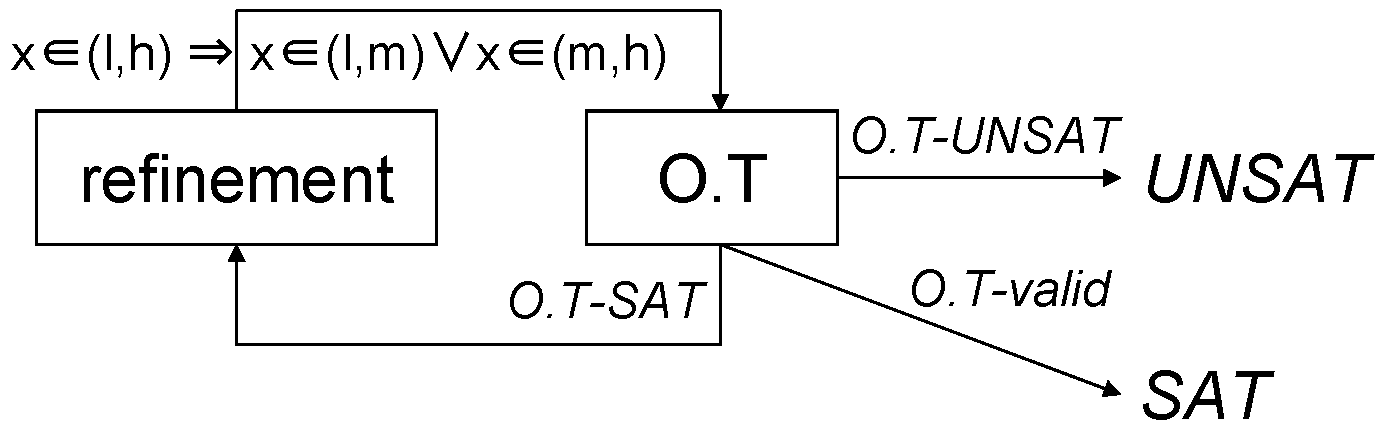
\includegraphics[height=0.6in,width=1.7in]{OTloop.png} & 
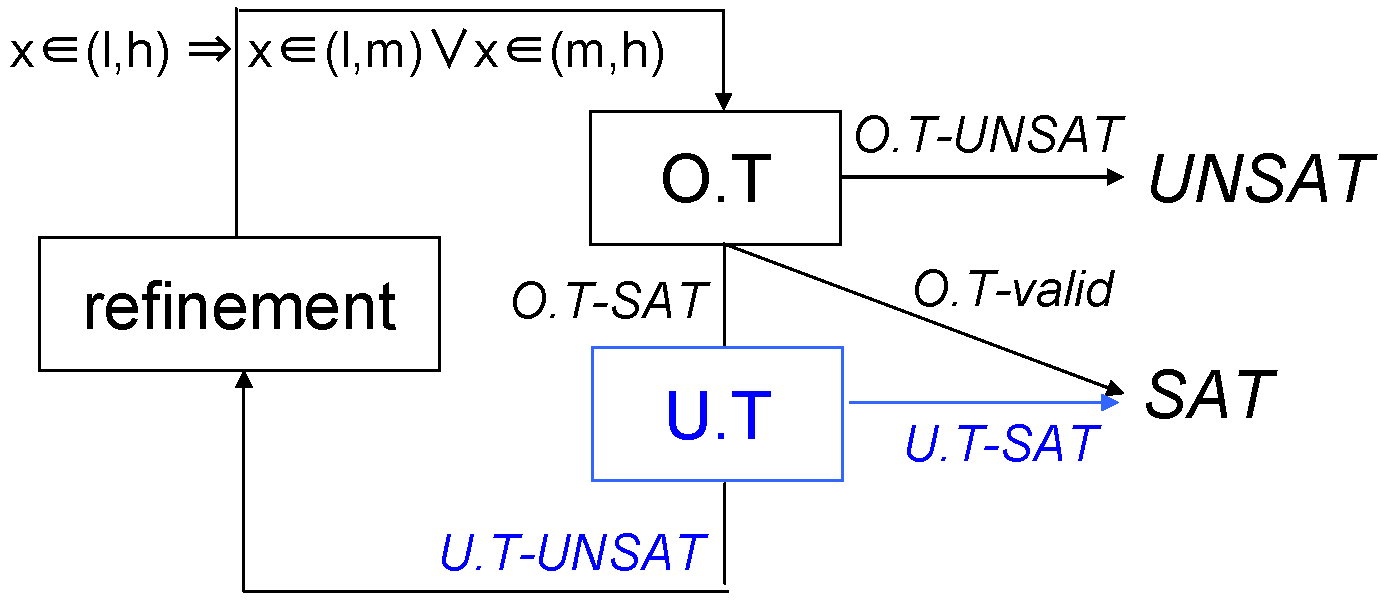
\includegraphics[height=0.9in,width=1.7in]{rasatloop.png} \\   
\mbox{(a) ICP loop} & \mbox{{\bf raSAT} loop} \\
\end{tabular}
\end{minipage} 
\caption{Refinement loops} 
\label{fig:OTrefine} 
\end{figure}
\end{comment}


\subsection{ICP Overview}
\sloppy  
Algorithm~\ref{Al:ICP} describes the basic ICP for solving polynomial inequalities
where two functions $prune(B,\psi)$ and $split(B)$ satisfy the following properties.
\begin{itemize}
\item If $B' = prune (B, \psi)$,
  then $B' \subseteq B $ and $ B' \cap \mathbb{S}(\psi) = B \cap \mathbb{S}(\psi)$. 
\item If $\{B_1, B_2\} = split (B)$,
  then $B = B_1 \cup B_2$ and $B_1 \cap B_2 = \emptyset$. 
\end{itemize}

\begin{figure}[hbt]
%\begin{minipage}[b]{1.0\linewidth}
\centering
\begin{tabular}{cc}
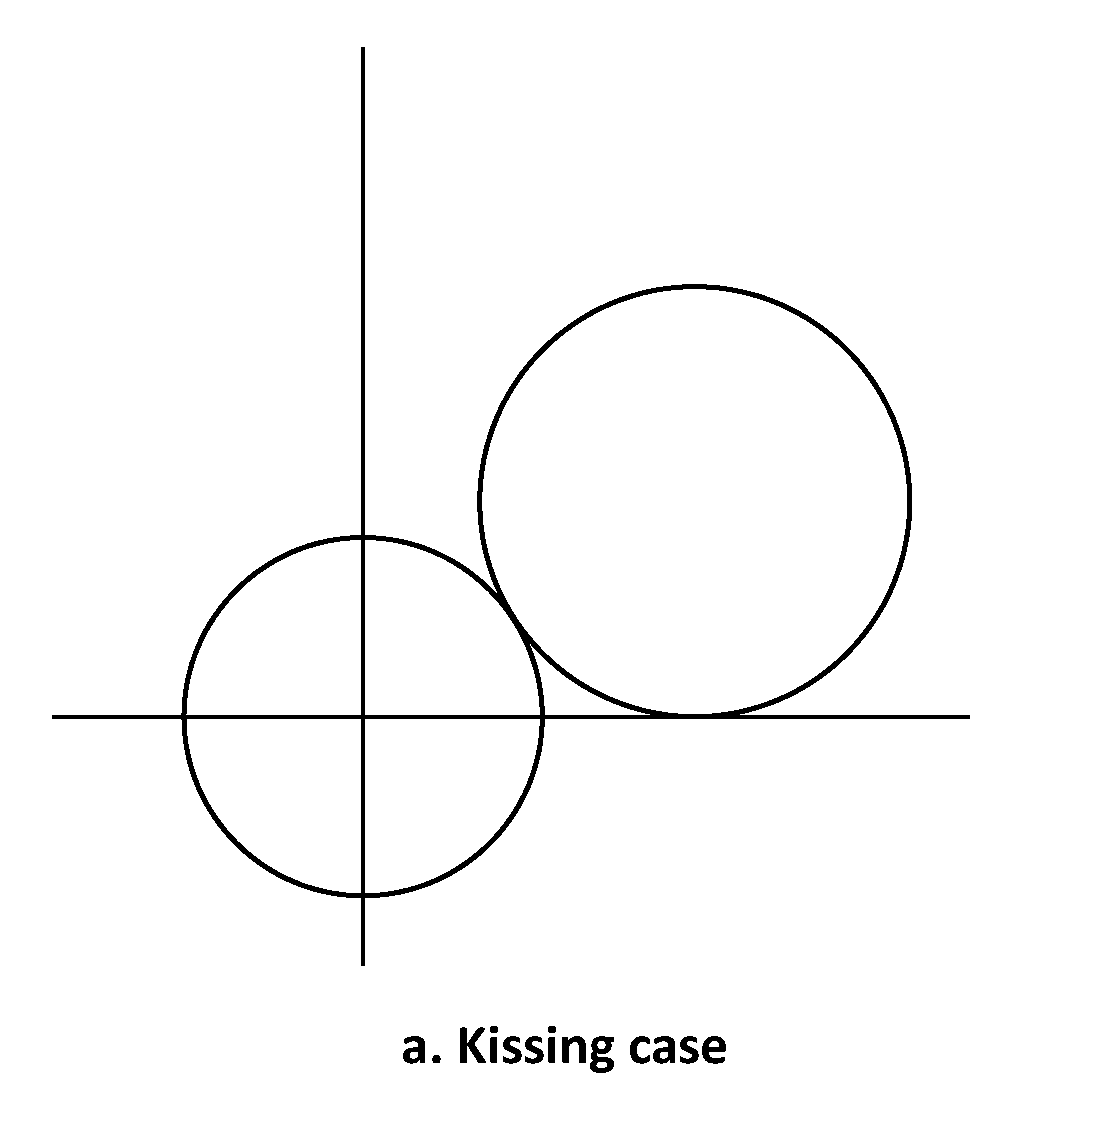
\includegraphics[height=1in,width=1.05in]{kissing.eps} &
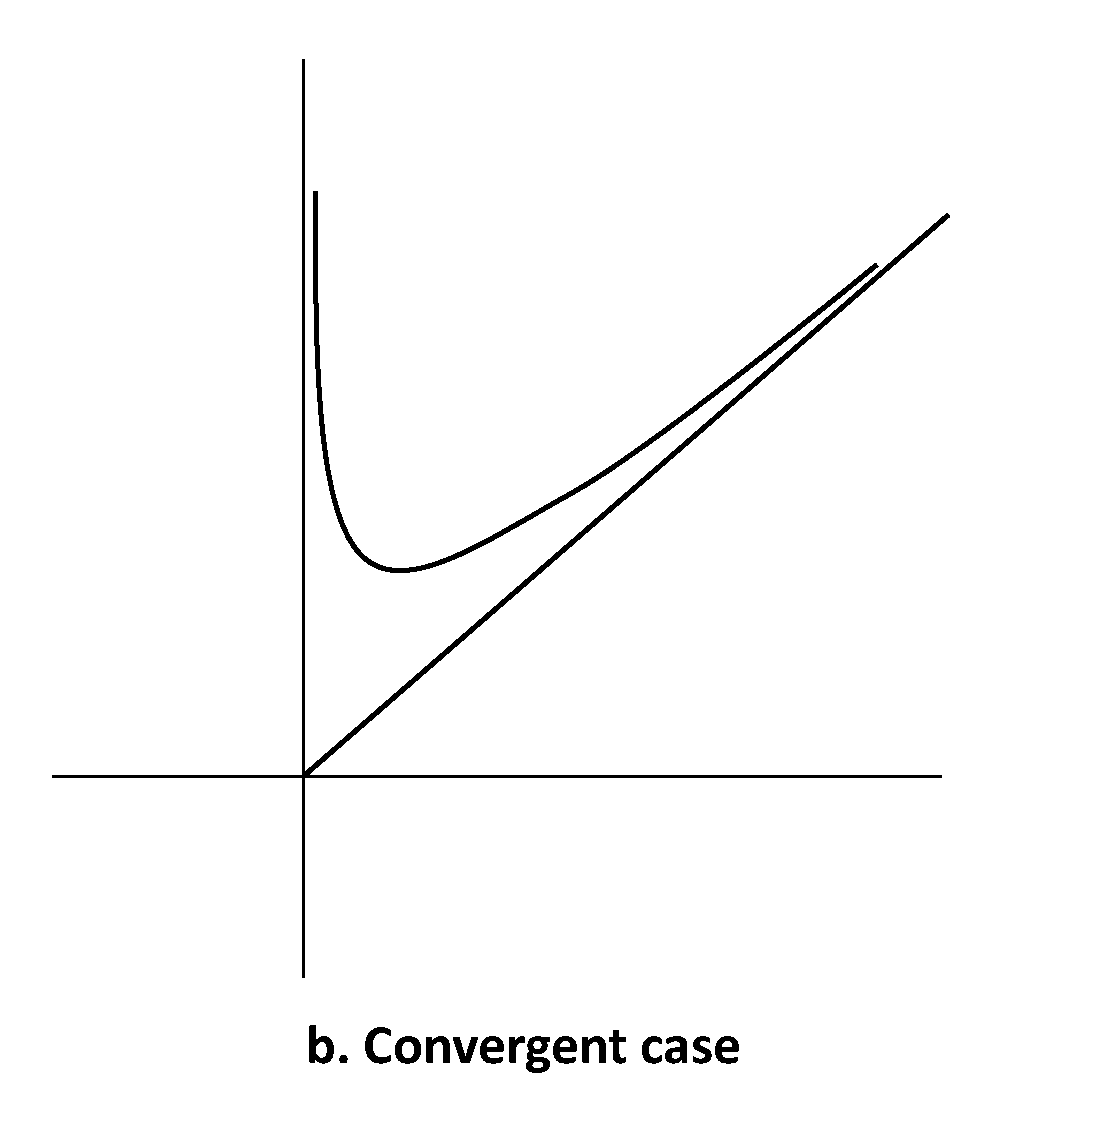
\includegraphics[height=1in,width=1.05in]{convergence.eps}
\end{tabular}
\caption{Limitations for detection of UNSAT} 
\label{fig:limit} 
%\end{minipage}
\end{figure} 

\noindent
ICP concludes SAT (line 8) only when it finds a box
in which the constraint becomes valid by IA. 
Although the number of boxes increases exponentially,
ICP always detects SAT of the inequalities 
$\psi$
if $I_1, \cdots, I_n$ are bounded. 
However, ICP may miss to detect UNSAT in cases of \emph{kissing} and
\emph{convergence} (Figure~\ref{fig:limit}).
\suppress{%%%%
The left shows a kissing case 
$x^2 + y^2 < 2^2 \wedge (x-4)^2 + (y-3)^2 < 3^2$ such that 
$\overline{\mathbb{S}(- x^2 - y^2 + 2^2 > 0)} \cap
 \overline{\mathbb{S}(- (x-4)^2 - (y-3)^2 + 3^2 > 0)} = \{(1.6, 1.2)\}$. 
Thus, it cannot be separated by the covering by (enough small) boxes. 
%Thus, there are no coverings to separate them. 
%$x^2 + y^2 < 2^2$ and $(x-4)^2 + (y-3)^2 < 3^2$. 
The right shows a convergent case 
$y > x + \frac{1}{x} \wedge y < x \wedge x > 0$,
i.e., $xy > x^2 + x \wedge y < x \wedge x > 0$.
The latter does not appear if all intervals are bounded. 
%The open box is $(0,\infty) \times (0,\infty)$ and 
%There are no finite coverings to separate them. 
%$y > x + \frac{1}{x}$ and $y < x$ for $x > 0$.
}


\begin{algorithm}
\begin{algorithmic}[1]
\State $S \gets \{B_0\}$ \Comment Set of boxes
\While {$S \neq \emptyset$}
  \State $B \gets S.choose()$ \Comment Get one box from the set
  \State $B' \gets prune(B, \psi)$
  \If {$B' = \emptyset$} \Comment The box does not satisfy the constraint
  	\State $S \gets S \setminus \{B\}$
  	\State continue
  \ElsIf {$B'$ satisfies $\psi$ by using \emph{IA}}
  	\State \Return SAT
  \Else \Comment \emph{IA} cannot conclude the constraint $\implies$ \emph{Refinement} Step
  	\State $\{B_1, B_2\} \gets split(B')$ \Comment split $B'$ into two smaller boxes $B_1$ and $B_2$	
  	\State $S \gets (S \setminus \{B\}) \cup \{B_1, B_2\}$
  \EndIf
\EndWhile
\State \Return UNSAT
\end{algorithmic}
\caption{ICP starting from the initial box $B_0 = I_1 \times \cdots \times I_n$}
\label{Al:ICP}
\end{algorithm}




%%%%%%%%%%
\suppress{
\begin{itemize}
\item if $\exists x_1 \in (a_1,b_1) \cdots x_n \in (a_n,b_n) . \wedge_{j} g_j > 0$ is SAT, 
ICP eventually detects it, and 
\item if $\exists x_1 \in [a_1,b_1] \cdots x_n \in [a_n,b_n] . \wedge_{j} g_j \geq 0$ is UNSAT, 
ICP eventually detects it, 
\end{itemize}
under the assumptions of fair decomposition and bounded intervals $(a_i,b_i)$ for all $i \in \{1, \cdots, n\}$. 
We will prepare terminology and briefly review this fact. 
}
%%%%%%%%%%%%
\suppress{
\begin{definition} \label{def:poly}
A polynomial inequality is a bounded quantification 
$\exists x_1 \in I_1 \cdots x_n \in I_n. \psi(x_1,\cdots,x_n)$ 
such that 
\begin{itemize}
\item each $I_i$ is an open interval $x_i \in (a_i,b_i)$, and 
\item $\psi(x_1,\cdots,x_n)$ is a conjunction of $f_j > 0$ 
where $f_j$ is a polynomial over $\{x_1, \cdots, x_n\}$. 
\end{itemize}
$f_i > 0$ is called an atomic polynomial inequality (API). 
We denote $\mathbb{S}(F) = \{x \in \Real^n \mid F ~\text{holds}\}$.
\end{definition}

\begin{example} \label{examp:poly_ieq}
$\exists x \in (-1,3)~y \in (2,4) . (x^3y - y^4 > 0) \wedge (y^3 -xy >0)$
is an example of a polynomial inequality with 2 variables and 2 APIs. 
\end{example}
}
%%%%%%%%%%%%%%%%%%%%%%

%%%%%%%%%%%%%%
\begin{comment}
\begin{definition}
An \emph{open box} of dimension $n$ is a set $(a_1,b_1) \times \cdots \times (a_n,b_n)$ 
where $a_i, b_i \in \Real, a_i \leq b_i$.  
For $\mathfrak{a} = (a_1, \cdots, a_n)$ and $\mathfrak{b} = (b_1, \cdots, b_n)$, 
we denote $(a_1,b_1) \times \cdots \times (a_n,b_n)$ by $(\mathfrak{a}, \mathfrak{b})$. 
\end{definition}

The set of all open boxes is a basis of Euclidean topology on $\Real^n$. 
In $\Real^n$, a set $U$ is compact if, and only if, $U$ is a bounded closed set. 
We denote a closure of a set $U$ by $\overline{U}$. 
%
Since a polynomial is continuous, 
$\mathbb{S}(\bigwedge \limits_{j=1}^m g_j > 0)$ is an open set. 
Note that $\Rat$ is dense in $\Real$, and an SAT instance in reals can be replaced with one in rationals. 

%%%%%%%%%%%%%%%%%%%%%%%%%%%%%%
\suppress{
\begin{lemma} \label{cor:rattoreal}
For a polynomial inequality
$F = \exists x_1 \in I_1 \cdots x_n \in I_n. \bigwedge \limits_{j=1}^m f_j > 0$, 
If there exists an SAT instance of F in $\Real^n$, there exists also in $\Rat^n$. 
\end{lemma}

\begin{lemma} \label{cor:refinement}
Suppose that $a_j < b_j$ for $1 \leq j \leq n$ and $f_i$'s are polynomials. 
Assume $a_k < c < b_k$ for some $k$. 
Then, 
$\exists x_1 \in (a_1,b_1) \cdots x_n \in (a_n,b_n). \bigwedge \limits_{i=1}^m f_i > 0$ 
is SAT (resp. UNSAT) if, and only if, 
$\exists x_1 \in (a_1,b_1) \cdots x_k \in (a_k,c) \cdots x_n \in (a_n,b_n). 
 \bigwedge \limits_{i=1}^m f_i > 0 
 \vee 
 \exists x_1 \in (a_1,b_1) \cdots x_k \in (c,b_k) \cdots x_n \in (a_n,b_n)). 
 \bigwedge \limits_{i=1}^m f_i > 0$ 
is SAT (resp. UNSAT). 
\end{lemma}

\begin{pf}
We show for the SAT case. If-part is obvious. For only-if-part, 
since $\mathbb{S}(\bigwedge \limits_{i=1}^m f_i > 0)$ is an open set, 
if $y \in (a_1,b_1) \times \cdots \{c\} \cdots \times (a_n,b_n)$ satisfies 
$\bigwedge \limits_{i=1}^m f_i > 0$, 
there exists $x_1 \in (a_1,b_1) \cdots x_k \in (a_k,c) \cdots x_n \in (a_n,b_n)$
(also $x_1 \in (a_1,b_1) \cdots x_k \in (c,b_k) \cdots x_n \in (a_n,b_n)$) that satisfies
$\bigwedge \limits_{i=1}^m f_i > 0$. 
\end{pf}

Lemma~\ref{cor:rattoreal} says that proving SAT of $F$ in $\Real$ is reduced to 
that in $\Rat$. 
Lemma~\ref{cor:refinement} says that, in the refinement step, we can apply refinement 
$x_k \in (a_k,b_k)$ to $x_k \in (a_k,c) \vee x_k \in (c,b_k)$, 
instead of $x_k \in (a_k,c] \vee x_k \in (c,b_k) $
(i.e., $c$ is ignored). 
}
%%%%%%%%%%%%%%%%%%%%%%%%%%%%%%

%Initially, interval constraints consists of conjunction only. Later, by refinements,
%it becomes a CNF. 

Note that an IA used in ICP is a converging theory. 

\begin{definition} \label{def:completeOT}
Let
$\varphi = \exists x_1 \in I_1 \cdots x_n \in I_n. \bigwedge \limits_{j=1}^m g_j > 0$
be a polynomial inequality such that each $I_i$ is bounded. 
An theory $T$ is {\em converging} 
if, for each $\delta > 0$ and $c = (c_1, \cdots, c_n) \in I_1 \times \cdots \times I_n$, 
there exists $\gamma > 0$ such that $T$ can concludes that  
for all $x_i \in (c_i - \gamma, c_i + \gamma)$, $i=1,\cdots, n$, we have 
 $\bigwedge \limits_{j=1}^m (g_j(c) - \delta < g_j(x) < g_j(c) + \delta)$. 
\end{definition}

%$O.T$ refinement loop is shown in Fig.~\ref{fig:OTrefine}~(a). 
%A standard ICP based algorithm of an SMT solver applies it with
%$O.T$ as a classical interval arithemtic. 
%The variation of interval arithemtic will be presented in Section~\ref{sec:approximation}. 

\begin{definition} 
Let
$\varphi = \exists x_1 \in I_1 \cdots x_n \in I_n. \bigwedge \limits_{j=1}^m g_j > 0$
for $I_i = (a_i,b_i)$.
A refinement strategy is {\em fair}, if, for each $c_i \in (a_i,b_i)$ and $\gamma > 0$, 
a decomposition of $I_i$ for each $i$ eventually occurs in $(c_i - \gamma, c_i + \gamma)$ 
(as long as neither SAT nor UNSAT is detected). 
\end{definition}

\begin{theorem} \label{th:RelComp}
Let
$\varphi = \exists x_1 \in I_1 \cdots x_n \in I_n. \bigwedge \limits_{j=1}^m g_j > 0$
for $I_i = (a_i,b_i)$.
Assume that
each $(a_i,b_i)$ is bounded, and a refinement strategy is fair. 
Then, 
\begin{itemize}
\item if $\exists x_1 \in (a_1,b_1) \cdots x_n \in (a_n,b_n) . \wedge_{j} g_j > 0$ is SAT, 
ICP eventually detects it, and
\item if $\exists x_1 \in [a_1,b_1] \cdots x_n \in [a_n,b_n] . \wedge_{j} g_j \geq 0$ is UNSAT, 
ICP eventually detects it.  
\end{itemize}
\end{theorem}


\begin{proof} 
The former is proved by the fact that, if $\varphi$ is SAT, there exists a non-empty neighborhood (open box) 
in $\cap~\mathbb{S}(g_j > 0)$. 
If the box decomposition strategy is fair, the refinement will eventually find such an open box. 

For the latter, assume that 
$\overline{\varphi} = \exists x_1 \in [a_1,b_1] \cdots x_n \in [a_n,b_n] . \wedge_{j} g_j \geq 0$ is UNSAT. 
Thus, $\cap~\overline{\mathbb{S}(g_j > 0)} = \emptyset$. 
Let $\delta_{j,k} = min \{|g_j(\bar{x}) - g_k(\bar{x})| \mid \bar{x} \in I_1 \times \cdots \times I_n\}$. 
Since $g_j$'s are continuous and $\overline{I_i}$'s are compact, $\delta_{j,k}$ is well defined,
and $\delta_{j.k} > 0$ for some $j,k$. 
Let $\delta = \frac{min \{ \delta_{j,k} \}}{2}$. 
Since IA is converging, there exists $\gamma > 0$ for $\delta > 0$ 
satisfying Definition~\ref{def:completeOT}, and fair decomposition eventually finds open boxes
such that $\mathbb{S}(g_j \ge 0)$ and $\mathbb{S}(g_k \ge 0)$ are separated. 
\qed
\end{proof}
\end{comment}
%%%%%%%%%%%%%%



\subsection{raSAT Loop}
ICP is extended to {\bf raSAT} loop~\cite{VanKhanh201227} which is displayed in Algorithm~\ref{Al:raSATLoop}.  
%Fig.~\ref{fig:OTrefine}~(b). 
\begin{algorithm}[h]
\begin{algorithmic}[1]
\While {$\Pi$ is satisfiable} \Comment Some more boxes exist
\State $\pi = \{x_i \in I_{ik} \mid i \in \{1,\cdots, n\}, k \in \{1,\cdots, i_k\} \} \gets $
a solution of $\Pi$ 	
\State $B \gets $ the box represented by
$\bigwedge\limits_{i=1}^n\bigwedge\limits_{k=1}^{i_k}x_i \in I_{ik}$

\If {$B$ does not satisfy $\psi$ by using \emph{IA}}
\State $\Pi \gets \Pi \wedge \neg(\bigwedge\limits_{i=1}^n\bigwedge\limits_{k=1}^{i_k}x_i \in I_{ik})$
  \ElsIf {$B$ satisfies $\psi$ by using \emph{IA}}
\State \Return SAT
  \ElsIf {$B$ satisfies $\psi$ by using \emph{testing}} \Comment Different from ICP
\State \Return SAT
\Else \Comment Neither \emph{IA} nor \emph{testing} conclude the constraint $\implies$
\emph{Refinement} Step
\State choose $(x_i \in I_{ik}) \in \pi$ such that $\forall k_1 \in \{1,\cdots, i_k\} I_{ik} \subseteq I_{ik_1}$
\State $\{I_1, I_2\} \gets split(I_{ik})$ \Comment split $I_{ik}$
into two smaller intervals $I_1$ and $I_2$
\State $\Pi \gets \Pi \wedge (x_i \in I_{ik} \leftrightarrow (x_i \in I_1 \vee x_i \in I_2))
\wedge \neg(x_i \in I_1 \wedge x_i \in I_2)$

\EndIf
\EndWhile
\State \Return UNSAT
\end{algorithmic}
\caption{\textbf{raSAT} loop starting from the initial box
  $\Pi = \bigwedge\limits_{i=1}^n x_i \in I_i^0$}
\label{Al:raSATLoop}
\end{algorithm}
%%%%%%%%%%%%%%
\begin{comment}
\begin{enumerate}
\item When an IA detects UNSAT (resp. valid), conclude UNSAT (resp. SAT). 
\item When an testing detects SAT, conclude SAT. 
\item If neither holds, a refinement is applied. 
\end{enumerate}
\end{comment} 
%%%%%%%%%%%%%
%
Its implementation {\bf raSAT} adapts various IAs including
Affine Interval~\cite{Comba93affinearithmetic,Ngoc:2009:ORE:1685167.1685421,VanKhanh201227} and Classical Interval (CI)~\cite{moore}. 
%which keep lower and upper bounds.
Although precision is incomparable, 
Affine Interval partially preserves the dependency among values, which is lost in CI. 
For instance, $x - x$ is evaluated to $[-2,2]$ for $x \in [2,4]$ by CI, but $0$ by an Affine Interval. 
More details can be found in~\cite{VanKhanh201227}.

\begin{comment}
Affine interval introduces \emph{noise symbols} $\epsilon$, 
which are interpreted as values in $(-1,1)$. 
For instance, $x = 3 + \epsilon$ describes $x \in (2,4)$, and 
$x - x = (3 + \epsilon) - (3 + \epsilon)$ is evaluated to $0$. 
The drawback is that the multiplication without dependency might be less precise than CI.
Affine intervals also cannot represent infinite intervals, e.g., $(0,\infty)$, 
since it becomes $\infty + \infty~\epsilon$. 
Forms of Affine intervals vary by choices how to approximate multiplications. They are,
\begin{enumerate}[(i)]
\item $\epsilon \epsilon'$ is replaced with a fresh noise symbol 
($AF$)~\cite{Comba93affinearithmetic}, 
\item $\epsilon \epsilon'$ is reduced to the fixed error noise symbol 
$\epsilon_{\pm}$ ($AF_1$ and $AF_2$) \cite{Messine_extensionsof},
\item $\epsilon \epsilon'$ is replaced with $(-1,1) \epsilon$ 
(or $(-1,1) \epsilon'$) ($EAI$)~\cite{Ngoc:2009:ORE:1685167.1685421},
\item $\epsilon \epsilon$ is reduced to fixed noise symbols 
$\epsilon_+$ or $\epsilon_{-}$ ($AF_2$) \cite{Messine_extensionsof}, 
\item Chebyshev approximation of $x^2$ introduces a noise symbol $|\epsilon|$ 
as an absolute value of $\epsilon$ with 
$\epsilon \epsilon = |\epsilon| |\epsilon| = |\epsilon| + (-\frac{1}{4}, 0)$ and
$\epsilon |\epsilon| = \epsilon + (-\frac{1}{4}, \frac{1}{4})$ \cite{VanKhanh201227}. 
%(Fig.~\ref{fig:chevabs}). 
%\item keeping products of noise symbols up to degree $2$ ($\epsilon_i \epsilon_j$),
\end{enumerate} 
\end{comment}

%%%%%%%%%%%%%%%%%
\suppress{
\begin{remark}
For Affine intervals, \emph{sensitivity}~\cite{ngocsefm} of a variable
is a possible range of the absolute value of the coefficient of its corresponding $\epsilon$. 

%In Example~\ref{examp:sensitivity}, $CAI$ estimates the coefficient of $|\epsilon_1|$ as $\textbf{3}$, 
%which has the largest sensitivity and indicates $x$ the most influencial. 

Note that Affine interval works only for bounded intervals. 
For instance, $\infty + \infty \epsilon$ represents $(-\infty,\infty)$, which says nothing. 
Narrowing intervals as an incremental search (Section~\ref{sec:incsearch})
partially depends on this fact. 
That is, if $\pm \infty$ is contained in an interval, first give finite upper/lower bounds and
search within these bounds using an Affine interval.
If UNSAT is concluded, then enlarge to the whole intervals using CI. 
\end{remark}
}
%%%%%%%%%%%%%%%%%


\begin{example} \label{examp:sensitivity}
Let $g = x^3 - 2xy$, $x = [0,2] = 1 + \epsilon_1$ and $y=[1,3] = 2+\epsilon_2$. While $AF_2$~\cite{VanKhanh201227} estimates the range of $g$ as 
$-3 - \epsilon_1 - 2\epsilon_2 + 3\epsilon_+ + 3\epsilon_{\pm}$ (thus $[-9,6]$),
$CAI$~\cite{VanKhanh201227} does as 
$[-4,-\frac{11}{4}] + [-\frac{1}{4}, 0]\epsilon_1 - 2\epsilon_2 +
 \textbf{3}|\epsilon_1| + [-2,2]\epsilon_{\pm}$ (thus $[-8,4.5]$).
\end{example}


%%%%%%%%%%%%%%%%%%%%%%%%%%
\suppress{
\begin{figure}[ht]
\begin{minipage}[b]{1.0\linewidth}
\centering
\begin{tabular}{ll}
\includegraphics[height=1.6in,width=1.7in]{chev1.pdf} &
\includegraphics[height=1.6in,width=1.7in]{chev2.pdf}
\end{tabular}
\caption{Chebyshev approximation of $x^2$ and $x~|x|$}
\label{fig:chevabs}
\end{minipage}
\end{figure}

$CAI$ \cite{tapas12} consists of (ii) and (v), which keeps better precision than iv)
for multiplications of the same variables, e.g., Taylor expansion. 
%To improve precision in estimating upper and lower bounds of polynomials, we apply 
%\textbf{Affine Arithmetic} such as $AF_1$, $AF_2$ \cite{af}, $CAI$ ~\cite{tapas12} 
%instead of Classical Interval \cite{moore}. 
%Note that upper and lower bounds estimated by IA are over-approximation bounds of polynomials.
}
%%%%%%%%%%%%%%%%%%%%%%%%%%
\suppress{
\begin{definition}
%For $\exists x_1 \in (a_1,b_1) \cdots x_n \in (a_n,b_n). \bigwedge \limits_{i=1}^m f_i(x_1,\cdots,x_n) > 0$, 
Let $M = \bigwedge \limits_{i=1}^m x_i \in (a_i,b_i)$ and 
${\mathcal P} = \bigwedge \limits_{i=1}^m f_i(x_1,\cdots,x_n) > 0$. 
%
Let $\delta_i^l$ and $\delta_i^u$ be lower and upper bounds of $f_i(x_1,\cdots,x_n)$ 
estimated by IA for $x_i \in (a_i,b_i)$. Then, we say 
%
%\vspace*{0.5em}
\begin{itemize}
\item ${\mathcal P}$ is \emph{IA-VALID} under $M$, if IA evaluates 
$~\forall i \in [1,m].~\delta_i^l > 0$,
%\vspace*{0.33em}
\item ${\mathcal P}$ is \emph{IA-UNSAT} under $M$, 
$~\exists i \in [1,m].~\delta_i^u \leq 0$, and 
\item ${\mathcal P}$ is \emph{IA-SAT} under $M$, if 
$(\exists j \in [1,m].~\delta_j^l \leq 0)\; \wedge \; 
	(\bigwedge \limits_{i=1}^m \delta_i^u > 0)$.
\end{itemize} 
\end{definition}

IA-VALID and IA-UNSAT safely reason satisfiability (SAT) and unsatisfiability (UNSAT), 
respectively. However, IA-SAT cannot conclude SAT. 
}
%%%%%%%%%%%%%%%%%



\section{SAT directed Strategies of {\bf raSAT}} \label{sec:strategy}

Performance of ICP is affected by the number of variables because the initial box 
$I_1 \times \cdots \times I_n$ will be decomposed into exponentially many boxes.
%since the decomposition phase would lead exponentially large number of boxes will be generated.
The detection of UNSAT requires exhaustive search on all boxes, and thus finding a small UNSAT core
is the key. 
For SAT detection, the keys will be a strategic control not to fall into local optimal and
a strategy to choose the most likely influential decomposition/box. 

\subsection{Incremental Search} \label{sec:incsearch}

Two incremental search strategies are prepared in {\bf raSAT}, 
(1) {\em incremental widening}, and (2) {\em incremental deepening}. 

\medskip \noindent 
\textbf{Incremental Widening.}
Given $0 < \delta_0 < \delta_1 < \cdots < \delta_k = \infty$, 
{\em incremental widening} starts with 
$B_0 =
[-\delta_0 , \delta_0] \times \cdots \times [-\delta_0 , \delta_0]$,
and if $\psi$ stays  UNSAT, then enlarge the box to 
$B_1 =
[-\delta_1 , \delta_1] \times \cdots \times [-\delta_1 , \delta_1]$. This continues until either SAT, timeout, UNSAT of
$B_k=
[-\delta_k , \delta_k] \times \cdots \times [-\delta_k , \delta_k]$. 
%
In {\bf raSAT}, $AF_2$ is used for $B_i$ if $i \neq k$, and $CI$ is used otherwise.



\begin{figure}[ht]
\begin{minipage}[b]{1.0\linewidth}
\centering
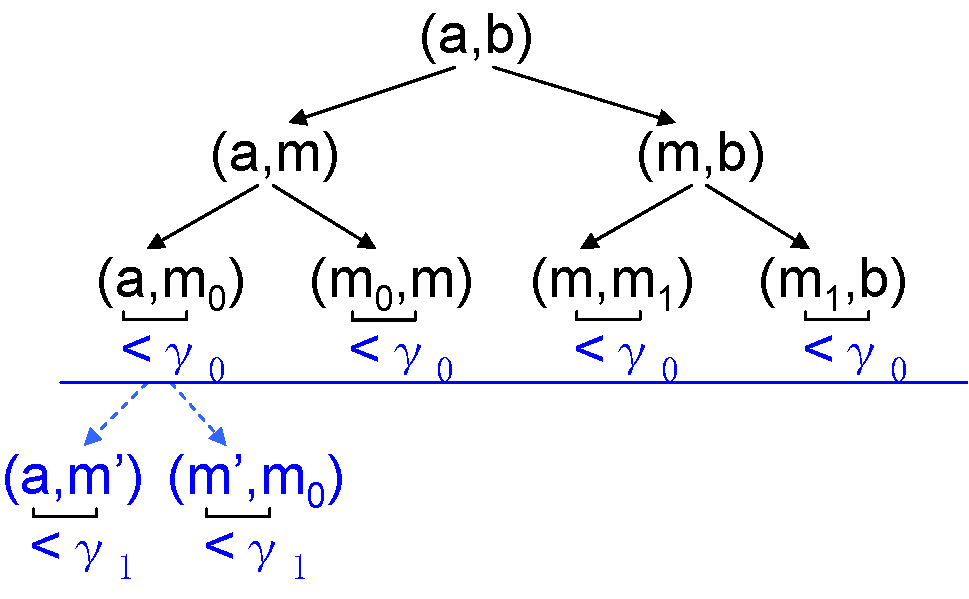
\includegraphics[height=1.2in,width=2in]{IncDeepen.png} \\
%\caption{Chebyshev approximation of $x^2$ and $x~|x|$}
\caption{Incremental Deepening}
\label{fig:incwid}
\end{minipage}
\end{figure}

\medskip \noindent 
\textbf{Incremental Deepening.}
To combine depth-first-search and breadth-first search among decomposed boxes,
{\bf raSAT} applied {\em incremental deepening}. 
Let $\gamma_0 > \gamma_1 > \cdots > 0$. 
It applies a threshold $\gamma$, such that no more decomposition occurs 
when a box becomes smaller than $\gamma$.
$\gamma$ is initially $\gamma=\gamma_0$. 
If neither SAT nor UNSAT is detected, {\bf raSAT} restarts with the threshold $\gamma_1$.
This continues until either SAT, timeout, or
a given bound of repetition is reached (Fig.~\ref{fig:incwid} (b)). 

\subsection{SAT Directed Heuristics Measure} \label{sec:SATheuristics}

%%%
\suppress{
With several hundred variables, we observe that an SMT solver works
when either SAT, or UNSAT with small UNSAT core.
%
For the latter, we need an efficient heuristics to find an UNSAT core, which is left as future work. 
For the former, the keys are how to choose variables to decompose, and 
how to choose a box to explore.
}%%%

In {\bf raSAT}, a strategy to select a variable to decompose is in the following two steps. 
(1) First select a least likely satisfiable {\em API} using {\em SAT-likelihood}, and
(2) then choose a most likely influential variable in such API using {\em sensitivity}.

\sloppy

In line 3 of Algorithm~\ref{Al:raSATLoop}, an IA estimates the range $range(g_j, B)$ of each polynomial $g_j$ in a box $B$. 
If an Affine Interval is used, the estimated range of $g_j$ is of the form
${[c_1,d_1]\epsilon_1 + \cdots + [c_n,d_n]\epsilon_n}$ from which $range(g_j, B)$ is obtained
by instantiating $[-1,1]$ to $\epsilon_i$. 
We have the following definitions. 
\begin{itemize} 
\item The {\em SAT-likelihood} of an API $g_j > 0$ is $| I \cap (0,\infty) | / |I|$
  for  $I = range(g_j, B)$. 
\item The {\em sensitivity} of a variable $x_i$ in an API $g_j > 0$ is $max(|c_i|, |d_i|)$. 
\end{itemize} 

\begin{example} \label{examp:SATlikelihood}
In Example~\ref{examp:sensitivity},  SAT-likelihood of $g$ is $0.4= \frac{6}{9-(-6)}$ by $AF_2$ 
and $0.36 = \frac{4.5}{4.5-(-8)}$ by $CAI$. The sensitivity of $x$ is $1$ by $AF_2$ and $3\frac{1}{4}$ by $CAI$,
  and that of $y$ is $2$ by both.
\end{example}


We define the {\em SAT-likelihood} of a box $B$ by 
the least SAT-likelihood of APIs. After a decomposition, {\bf raSAT} simply compares SAT-likelihood of newly decomposed boxes with those of previous ones to select one box to explore.

\medskip \noindent \sloppy
\textbf{Test Case Generation Strategy.}
The sensitivity of variables is further used in test case generation where
%That is, {\bf raSAT} generates two test cases for the specified number of variables,
%and one for the rest. 
%Such variables are selected from those with larger sensitivity.
%When two test cases are generated, 
{\bf raSAT} observes
the sign of the coefficients of noise symbols.
If positive, it takes the upper bound of possible values as the first test case; 
otherwise, the lower bound. %The second test case is generated randomly. 

%We perform experiments only on inequations of Zankl, and Meti-Tarski families. 
The effects of designed strategies are examined on Zankl and Meti-Tarski families of \emph{QF\_NRA}, which are illustrated in
Table~\ref{tab:rasat-experiments}. A brief comparison with ICP-based solvers is also presented in the table where UNSAT of \textbf{raSAT} and \textbf{dReal} is over $[-\infty, \infty]$ while that of \textbf{iSAT3} is over $[-1000, 1000]$ (otherwise \textbf{iSAT3} often causes segmentation faults with $[-\infty, \infty]$). In addition, \textbf{dReal} concludes either $\delta-$SAT which cannot imply SAT, or UNSAT.
The experiments are done on a machine with Intel Xeon E5-2680v2 2.80GHz and 4 GB of RAM. The timeout is set to 500s, and time shows the total of successful cases 
(either SAT or UNSAT). %Our combinations of strategies are,




\begin{table}[ht]
\begin{center}
\adjustbox{max width=\columnwidth}{
\begin{tabular}{ | l | r | r | r | r | r | r | r | r |  r | r | r | r | r | r | r | r |}
\hline
    \multirow{2}{*}{Benchmark} & \multicolumn{4}{c|}{Random} &
    \multicolumn{4}{c|}{Strategy}&
        \multicolumn{4}{c|}{iSAT3} &
            \multicolumn{4}{c|}{dReal}\\
    \cline{2-17}
    &\multicolumn{2}{c|}{SAT}&\multicolumn{2}{c|}{UNSAT}&\multicolumn{2}{c|}{SAT}&\multicolumn{2}{c|}{UNSAT}&\multicolumn{2}{c|}{SAT}&\multicolumn{2}{c|}{UNSAT}&\multicolumn{2}{c|}{$\delta-$SAT}&\multicolumn{2}{c|}{UNSAT}\\
\hline
    Zankl & 20 & 243.82 (s) & 10 & 0.38(s) & \textbf{36} & 1679.76(s) &  10 & 0.39(s) & 14 & 201.08(s) & \textbf{15} & 8.06 (s) & 65 & 6282.32(s) & 0 & 0(s)
\\
\hline
    Meti-Tarski & 3451 & 895.14 (s) &1060 & 233.46 (s) & \textbf{3473} & 419.25 (s) & 1052 & 821.85 (s) & 2916 & 811.53(s) & \textbf{1225} & 73.83 (s) & 3523 & 441.35 (s) & 1197 & 55.39 (s)
\\
\hline
\end{tabular}
}
\end{center}
\caption{Effectiveness of Heuristics} 
\label{tab:rasat-experiments}
\end{table}


\section{Extension for Equations Handling} \label{sec:eq}
\begin{comment}
For a polynomial constraint with equations,
\[\psi =
\bigwedge \limits_{j=1}^m g_j > 0 \wedge
\bigwedge \limits_{j=m+1}^{m'} g_j = 0\]
one typical way to solve equations is an algebraic method, e.g., Groebner basis.
\end{comment}
In this section, we try a simple method based on
the {\em Intermediate Value Theorem} which is illustrated by cases of single equation and multiple ones.

\medskip \noindent 
\textbf{Single Equation.}
A single equation (${g=0}$) can be solved in a simple way by finding 2 test cases with $g > 0$ and $g < 0$, which implies 
$g=0$ somewhere in between. 

\begin{lemma} \label{lemma:ivt}
For $\psi =
\bigwedge \limits_{j=1}^m g_j > 0~\wedge~g = 0$.
Suppose a box
$B$
and
%where
%for all $i \in \{1, \cdots, n\}$,
let ${[l_g, h_g] = range(g, B)}$, 
\begin{enumerate}[(i)]
\item If $l_g > 0$ or $h_g < 0$, then $g = 0$ is UNSAT in $B$ and thus that is for $\psi$.
\item If $\bigwedge \limits_{j=1}^m g_j > 0$ is IA-valid in $B$ and there are $\vec{t},\vec{t'} \in B$
  with $g(\vec{t}) > 0$ and $g(\vec{t'}) < 0$, then $\psi$ is SAT.
\end{enumerate}
\end{lemma}

%%%%%%%%%%%%%
\suppress{
\begin{proof}
\begin{enumerate}[(i)]
\item If $l_g > 0$ or $h_g < 0$, then $g=0$ cannot be satisfied in box $I$.
  As a result, $F$ is UNSAT in $I$. 
\item If there are two instances $\vec{t},\vec{t'}$ in the box with
  $g(\vec{t}) > 0$ and $g(\vec{t'}) < 0$, it is clear from the Intermediate
  Value Theorem that there exist one point $\vec{t_0}$ between $\vec{t}$ and
  $\vec{t'}$ such that $g(\vec{t_0}) = 0$. In addition, because
  $\bigwedge \limits_{j}^m f_j > 0$ is IA-VALID in $I$, $\vec{t_0}$ also
  satisfies $\bigwedge \limits_{j}^m f_j > 0$.
  As a result, $F$ is satisfiable with $\vec{t_0}$ as the SAT instance.
\end{enumerate}
\end{proof}
}
%%%%%%%%%%%%
If neither (i) nor (ii) holds, \textbf{raSAT} continues the decomposition.
\begin{example}
  Let $\varphi = f(x, y) > 0 \wedge g(x, y) = 0$.
  Suppose we find a box 
  ${B = [a, b] \times [c, d]}$
  such that $f(x, y) > 0$ is IA-VALID in $B$.
  (Fig.~\ref{fig:single-equation}).
  In addition, 
  if we find two points $(u_1, v_1)$ and $(u_2, v_2)$ in $B$ such that
  $g(u_1, v_1) > 0$ and $g(u_2, v_2) < 0$,
  then the constraint is satisfiable by Lemma~\ref{lemma:ivt}. 
\end{example}


\begin{figure}
\centering
\begin{subfigure}{0.4\textwidth}
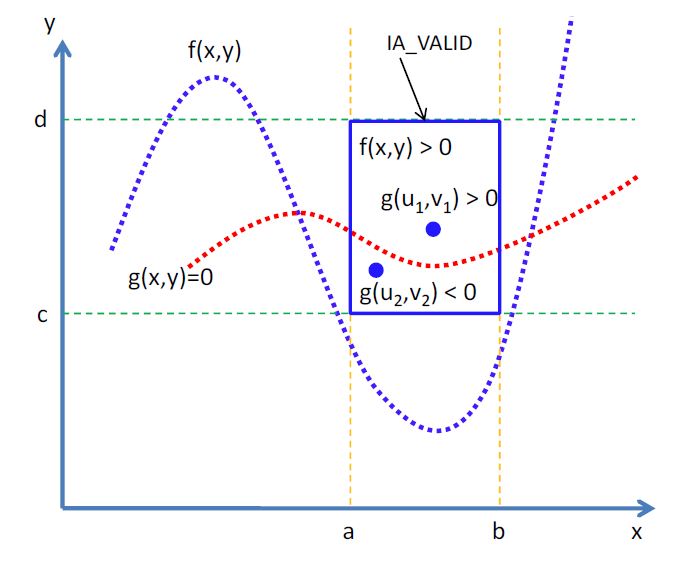
\includegraphics[width=1.\linewidth]{singleEquation.png} 
\caption{Single equation}
\label{fig:single-equation}
\end{subfigure}
\begin{subfigure}{0.4\textwidth}
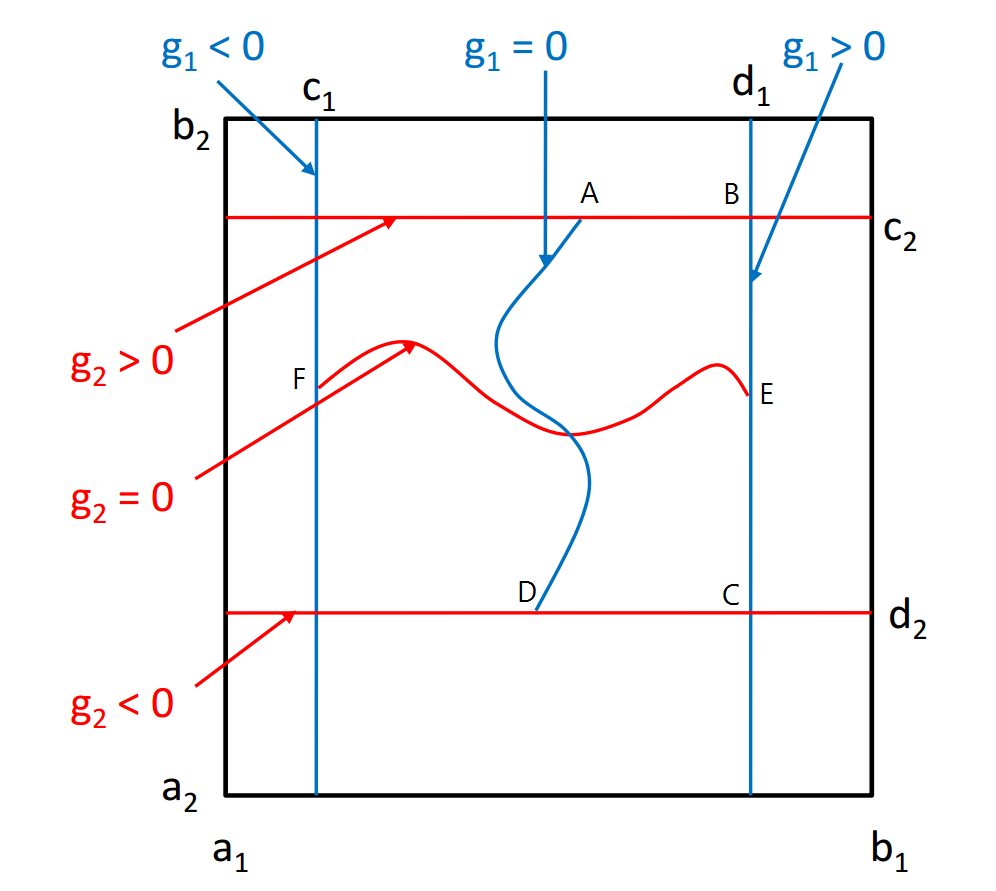
\includegraphics[width=1.\linewidth]{multipleEquations.png}  
\caption{Multiple equations}
\label{fig:multiple-equations}  
\end{subfigure}
\caption{Example on solving equations using the Intermediate Value Theorem}
%\end{minipage}
\end{figure}

\medskip \noindent 
\textbf{Multiple Equations.}
The above idea is extended for solving multiple equations. 
Consider $m$ equations ($m \ge 1$): $\bigwedge \limits_{j=1}^m g_j = 0$ and 
an box $B = {[l_1, h_1] \times \cdots [l_n, h_n]}$.
Let ${V = \{v_1, \cdots, v_n\}}$ be the set of variables. For $V' = \{x_{i_1}, \cdots x_{i_k} \} \subseteq V$,
we denote $B\downarrow_{V'}$ and $B\uparrow_{V'}$ as $\{ (r_1, \cdots, r_n) \in B \mid r_i = l_i~\text{for }i=i_1,...,i_k \}$
and ${\{ (r_1, \cdots, r_n) \in B \mid r_i = h_i~\text{for }i=i_1,...,i_k \}}$, respectively. 

\begin{definition} \label{def:CheckBasis} 
A sequence $(V_1, \cdots, V_m)$ of subsets of $V$ is a {\em check basis} of $(g_1, \cdots, g_m)$ on a box $B$,
if, for each $j,j'$ with $1 \leq j, j' \leq m$, 
\begin{enumerate}
\item $V_j (\neq \emptyset) \subseteq var(g_j)$, 
\item $V_j \cap V_{j'} = \emptyset$ if $j \neq j'$, and 
\item either $g_j > 0$ on $B\uparrow_{V_j}$ and $g_j < 0$ on $B\downarrow_{V_j}$, or
      $g_j < 0$ on $B\uparrow_{V_j}$ and $g_j > 0$ on $B\downarrow_{V_j}$. 
\end{enumerate}
\end{definition} 
%%%
\suppress{
For all $j\in \{1, \cdots, m\}$, let $k_j = |V_j|$ and
${V_j = \{v_{jk} \mid 1 \le k \le k_j \}}$, then, there exist two combinations
${(x_{j1}, \cdots, x_{jk_j}) = (t_{j1}, \cdots, t_{jk_j})}$ and
${(x_{j1}, \cdots, x_{jk_j}) = (t'_{j1}, \cdots, t'_{jk_j})}$
where $t_{jk} \neq t'_{jk} \in (l_{jk}, h_{jk})$, $1 \le k \le k_j$ such that
\[g_j(t_{j1}, \cdots, t_{jk_j}, \cdots, x_{jk}, \cdots) > 0\] and
\[g_j(t'_{j1}, \cdots, t'_{jk_j}, \cdots, x_{jk}, \cdots) < 0\]
for all values of $x_{jk}$ in $(l_{jk}, h_{jk})$ where $x_{jk} \in var(g_j) \setminus V_j$.
We denote $ivt(g_j, V_j, I)$ to represent that the polynomial $g_j$ enjoy this property
with respect to $V_j$ and $I$.
} %%%

\begin{lemma} \label{lem:multieq}
For a polynomial constraint containing multiple equations \[\psi= 
\bigwedge \limits_{j=1}^m g_j>0 \wedge
\bigwedge \limits_{j=m+1}^{m'} g_j = 0\]
and a box $B$, 
assume that
\begin{enumerate}
\item $\bigwedge \limits_{j=1}^m g_j>0$ is IA-valid on $B$, and
\item there is a {\em check basis} $(V_{m+1}, \cdots, V_{m'})$ of $(g_{m+1}, \cdots, g_{m'})$ on B. 
\end{enumerate}
Then, $\psi$ has a SAT instance in $B$.
\end{lemma}

The idea is, from the Intermediate Value Theorem,
each $j \in \{m+1, \cdots, m'\}$, $g_j$ has a $n - |V_{j}|$ dimensional surface of null points of $g_j$
between $B\uparrow_{V_j}$ and $B\downarrow_{V_j}$. 
Since $V_j$'s are mutually disjoint (and $g_j$' are continuous),
we have the intersection of all such surfaces of null points with
the dimension $n - \sum_{j=m+1}^{m'} |V_j|$.
Thus, this method has a limitation that 
the number of variables must be greater than or equal to the number of equations.

\begin{example}
  Consider two equations $g_1(x, y)=0$ and $g_2(x, y) = 0$, and assume that $(\{x\}, \{y\})$
  is a check basis of $(g_1, g_2)$ on $[c_1,d_1] \times [c_2,d_2]$ (Fig.~\ref{fig:multiple-equations}).
  Then, the blue line (null points of $g_1$) and the red line (null points of $g_2$) must have
  an intersection. We can explain this by Jordan curve theorem. 
  Since $ABCD$ is a closed curve such that $E$ is inner and $F$ is outer,
  a continuous (red) line $EF$ must have an intersection by Jordan curve theorem. 
\end{example}

\begin{comment}
Current {\bf raSAT} for polynomial constraints with equations is implemented in a naive way. 
For instance, for each $g_j = 0$, \textbf{raSAT} checks all possible subsets of its variables
as candidates for $V_j$. Thus, in the worst case \textbf{raSAT} checks
$2^{|var(g_1)|}*\cdots*2^{|var(g_m)|}$ cases.
It also does not prepare a strategy to find a box that makes all inequations IA-valid.
Preliminary experiments on problems with equations from QF\_NRA/Zankl and QF\_NRA/Meti-tarski
are summarized in Table~\ref{tab:equations}.
We hope that the sensitivity will give effective strategies. 
\end{comment}

\begin{comment}
\begin{table*}[hbt]
\centering
\adjustbox{max width=\columnwidth}{
\begin{tabular}{ | l | r | r | r | r  | r | r | r | r | r | r |r | r | r | r | r | r |}
\hline
    \multicolumn{1}{|l|}{Benchmark} & 
    \multicolumn{4}{c|}{\bf raSAT} & \multicolumn{4}{c|}{\bf Z3 4.3} & \multicolumn{4}{c|}{\bf iSAT3} & \multicolumn{4}{c|}{\bf dReal}\\
\hline
    & \multicolumn{2}{c}{SAT} & \multicolumn{2}{|c}{UNSAT} & \multicolumn{2}{|c}{SAT} 
    & \multicolumn{2}{|c}{UNSAT} & \multicolumn{2}{|c}{SAT} & \multicolumn{2}{|c}{UNSAT} & \multicolumn{2}{|c}{$\delta-$SAT} & \multicolumn{2}{|c|}{UNSAT}\\
\hline
Zankl (15) & \textbf{11} & 0.07 (s) & \textbf{4} & 0.17 (s) & \textbf{11} & 0.17 (s) & \textbf{4} & 0.02 (s) & 0 & 0.00 (s) & \textbf{4} & 0.05 (s) & 11 & 0.06 (s) & \textbf{4} & 0.02(s)\\
\hline
Meti-Tarski (3528/1573) & 875 & 174.90 (s) & 781 & 401.15 (s) & \textbf{1497} & 21.00 (s) & \textbf{1115} & 74.19 (s) & 1 & 0.28 (s) & 
1075 & 22.6 (s) & 1497 & 72.85 (s) & 943 & 21.40 (s) \\
\hline
Keymaera (612) & 0 & 0.00 (s)& 312 & 66.63 (s) & 0 & 0.00 (s) & \textbf{610} & 2.92 (s) & 0 & 0.00 (s) & 226 & 1.63 (s) & 13& 4.03 (s) & 318 & 1.96 (s) \\
\hline 
\end{tabular}
}
\medskip 
\caption{Comparison among SMT solvers with equations} \label{tab:equations}
\end{table*}
\end{comment}

%%%%%%
\suppress{
\begin{algorithm}
\begin{algorithmic}[1]
\Function{equationsProver}{$\bigwedge\limits_{j=k}^mg_j = 0, \Pi, V_0$}
\If {$k > m$} \Comment{All equations are checked}
	\State \Return SAT
\EndIf
\For {$V_k \in P(var(g_k))$} \Comment{$P(var(g_k))$ is the powerset of $var(g_k)$}
	\If {$V_k \cap V = \emptyset$ and $ivt(g_k, V_k, \Pi)$}
		\State $V_0 \gets V_0 \cup V_k$
		\If {\Call{equationsProver}{$\bigwedge\limits_{j=k+1}^mg_j = 0, \Pi, V_0$} = SAT}
			\State \Return SAT
		\EndIf
	\EndIf
\EndFor
\State \Return UNSAT
\EndFunction
\State \Call{equationsProver}{$\bigwedge\limits_{j=1}^mg_j = 0, \Pi, \emptyset$}
\end{algorithmic}
\caption{Solving multiple equations $\bigwedge\limits_{j=1}^m g_j = 0$ with ${\Pi = \bigwedge\limits_{i = 1}^n x_i \in (l_i, h_i)}$}
\label{Al:multiple-equations}
\end{algorithm}
}%%%%%% 




\section{Conclusion} \label{sec:conclusion and Future Work}

This paper presented {\bf raSAT} loop, which extends ICP with testing to accelerate
SAT detection and implemented as an SMT solver \textbf{raSAT}. 
With experiments on benchmarks from QF\_NRA of SMT-LIB, we found two heuristic measures, 
{\em SAT-likelihood} and {\em sensitivity}, which lead an effective strategy for SAT detection. 
%Currently, {\bf raSAT} is in proto-type status, and lots of future work remain. 

We have some ideas for the future works.

%
\suppress{
\subsection{Observation and Discussion} 

From experimental results in Section~\ref{sec:experiments} and~\ref{sec:expsmtlib}, 
we observe the followings. 
\begin{itemize}
\item The degree of polynomials will not affect much. 
\item The number of variables are matters, but also for Z3 4.3. 
The experimental results do not show exponential growth, and we expect 
the strategy of selection of an API in which related intervals are decomposed
seems effective in practice. By observing Zankl examples, we think the maximum 
number of variables of each API seems a dominant factor. 
\item Effects of the number of APIs are not clear at the moment. In simple benchmarks, 
{\bf raSAT} is faster than Z3 4.3, however we admit that we have set small degree $n=6$
for each API. 
\end{itemize}

For instance, {\em matrix-2-all-5,8,11,12} in Zankl 
contain a long monomial (e.g., $60$) with the max degree $6$, and 
relatively many variables (e.g., $14$), which cannot be solved by Z3 4.3, but 
{\bf raSAT} does. 
As a general feeling, if an API contains more than $30 \sim 40$ variables, 
{\bf raSAT} seems saturating. 
We expect that, adding to a strategy to select an API (Section~\ref{sec:intervaldecomp}), 
we need a strategy to select variables in the focus. We expect this can be designed 
with sensitivity (Example~\ref{examp:sensitivity}) and would work in practice. 
Note that sensitivity can be used only with noise symbols in Affine intervals. 
Thus, iSAT and RSOLVER cannot use this strategy, though they are based on IA, too. 

\subsection{Future Work}
}
%

\noindent 
{\bf UNSAT Core}. Currently, \textbf{raSAT} focuses on SAT detection. For
UNSAT detection, the target is to find a small UNSAT core in a large problem.


\noindent 
{\bf Equations Handling}. 
Section~\ref{sec:eq} shows incomplete equations handling, %but current implementation has no effective strategies
%on finding a decomposition $V_j$'s. 
%We hope to find one based on the sensitivity.
we would like to additionally apply Groebner basis
to overcome the limitation that
the number of variables is greater-than-equal to that of equations.

%%%%
\suppress{
where UNSAT constraints can be completely solved by ICP (with the assumption of bounded intervals).
The Intermediate Value Theorem can be used to show satisfiability with restrictions on variables of polynomials.
Moreover, the use of this theorem is not complete in showing satisfiability.
As a future work, we will apply
Groebner basis in addition to the current use of the Intermediate Value Theorem.
}
%%%%

%\medskip \noindent 
%{\bf Further strategy refinement}. 
%Currently, raSAT uses information only from IA. We hope to refine strategies such that previous
%IA and testing results mutually guide. For instance, a box decomposition strategy can be a target.

%%%
\suppress{
\subsubsection{Extension of {\bf raSAT} loop}
\begin{itemize}
\item {\bf Equality handling}: currently, {\bf raSAT} loop can handle only inequalities. 
Before applying ideal based technique, such as {\em Gr{\"o}bner basis}, 
we are planning to implement a non-constructive detection of equality 
by {\em intermediate value theorem}. 

\suppress{
\item{\textbf{Polynomial equality by Intermediate value theorem}:} 
Consider 
\begin{center}
$(x_1 \in (a_1,b_1) \wedge \cdots \wedge x_n \in (a_n,b_n))~\bigwedge 
\limits_{j}^m f_j(x_1,\cdots,x_n) > 0~\wedge~g(x_1,\cdots, x_n) = 0.$
\end{center}
SAT can be proved by two steps. First, find a box of the product of 
$(l_{ik},h_{ik}) \subseteq (l_i,h_i)$ (by the IA) such that 
\begin{center}
$\forall x_1 \in (l_{1k},h_{1k}) \cdots x_n \in (l_{nk},h_{nk}).~\bigwedge 
 \limits_{j}^m f_j(x_1,\cdots,x_n) > 0$~~~~(IA-VALID) 
\end{center}
and find two instances (by testing) in the box with $g(a_1,\cdots,a_n) > 0$ 
and $g(b_1,\cdots,b_n) < 0$. By Intermediate value theorem, we can conclude 
$\exists x_1 \in (l_1,h_1) \cdots x_n \in (l_n,h_n).~g(x_1,\cdots, x_n) = 0$. 
}

\item \textbf{Solving polynomial constraints on integers}: 
In integer domain, the number of test data is finite if intervals are bounded. 
Then, Test-UNSAT implies UNSAT if all possible test data are generated. 
A tight interaction between testing and interval decomposition could be investigated.
Mixed integers are also challenging. 
\end{itemize}


\subsubsection{\textbf{raSAT} Development}

\begin{itemize}
\item \textbf{Avoiding local optimal}: 
we borrow an idea of \emph{restart} in MiniSAT for escaping from hopeless local search 
(i.e., solution set is not dense or empty). 
\emph{Heuristics} would be, after a deep interval decomposition of 
a box and Test-UNSAT are reported, backtrack occurs to choose a randomly selected box. 

\item \textbf{Separation of linear constraints}: 
Many benchmarks contain linear constraints. Current implementation does not have 
any tuning, but {\bf raSAT} loop only. 
Practically, separating linear and non-linear constraints and solving them 
in a coordinated way between Presburger arithmetic and {\bf raSAT} would improve. 
During this separation, variables of intersecting linear constraints would be candidates 
for interval decomposition. 

\item \textbf{Incremental DPLL}: For interactions with the SAT solver, 
we currently apply the very lazy theory learning. Combination with 
\emph{eager} theory propagation would improve, in which we can propagate 
a conflict from a partial truth assignment instead of waiting 
for a full truth assignment obtained by SAT solver.
\end{itemize}
}
%%

%%
\suppress{
\subsection{Applications}
\begin{itemize}
\item \textbf{Checking overflow and roundoff error}: In the computers, the real numbers are represented by finite numbers (i.e., floating point numbers, fixed point numbers). Due to finite representation, the over-flow and roundoff errors (OREs) \cite{ngocsefm, ngocase} may occur. The OREs will be propagated through computations of the program. Further, the computations themselves also cause OREs because the arithmetic needs to round the result to fit the number format. Besides, OREs are also affected by types of statements, i.e., branch, loop, assignment statements.
By symbolic execution, ORE constraints are propagated from a program and ORE problems are reduced to problems of solving ORE constraints for verifying whether OREs occur. 
%For solving ORE constraint, combination of the new form of affine arithmetic ($CAI_1$) and \emph{sensitivity} (i.e., high degrees, )

\item \textbf{Loop invariant generation}: The problem of linear invariant generation is often reduced to the problem of non-linear constraint solving. 
Since Farkas's Lemma \cite{Colon03} uses the product of matrices with polynomial constraint solving, we can extend the target for non-linear invariant generation.
%Based on Farkas' Lemma \cite{Colon03}, non-linear constraints on coefficients of the target linear invariant are generated and a satisfiable instance of these constraints is a candidate of the linear invariant. 
\end{itemize}
}
%%


%\balance
\bibliographystyle{splncs03}
\bibliography{generic}
\begin{comment}
\begin{thebibliography}{10}
\providecommand{\url}[1]{\texttt{#1}}
\providecommand{\urlprefix}{URL }

\bibitem{Al2012.14}
Alliot, J.M., Gotteland, J.B., Vanaret, C., Durand, N., Gianazza, D.:
  {Implementing an interval computation library for OCaml on x86/amd64
  architectures}. {ICFP}, ACM (2012)

\bibitem{benhamou:hal-00480814}
  Benhamou, F., Granvilliers, L.: {Continuous and Interval Constraints}.
  {Handbook of Constraint Programming} (2006), pp.571--604

\bibitem{Barcelogic08}
 Bofill, M., Nieuwenhuis, R., Oliveras, A., Rodríguez-Carbonell, E., Rubio, A.:
 {The Barcelogic SMT solver}. CAV 2008. LNCS 5123. pp.294--298 (2008)
  
\bibitem{Bryant07decidingbit-vector}
  Bryant, R.E., Kroening, D., Ouaknine, J., Seshia, S.A., Strichman, O., Brady, B.:
  Deciding bit-vector arithmetic with abstraction. TACAS 2007.
  LNCS 4424, pp. 358--372 (2007)

\bibitem{qecad}
  Collins, G.: Quantifier elimination by cylindrical algebraic decomposition
  - twenty years of progress. Quantifier Elimination and Cylindrical
  Algebraic Decomposition, pp. 8--23 (1998)

%\bibitem{Colon}
%Colón, M., Sankaranarayanan, S., Sipma, H.: Linear invariant generation using
%  non-linear constraint solving. 
%  CAV, LNCS 2725, pp. 420--432
%  (2003)
  
\bibitem{Comba93affinearithmetic}
Comba, J.L.D., Stolfi, J.: Affine arithmetic and its applications to computer
  graphics (1993)

\bibitem{smtrat}
Corzilius, F., Loup, U., Junges, S., Ábrahám, E.: Smt-rat: An SMT-compliant
  nonlinear real arithmetic toolbox. SAT 2012, vol. 7317, pp. 442--448

\bibitem{isat}
Fränzle, M., Herde, C., Teige, T., Ratschan, S., Schubert, T.: Efficient
  solving of large non-linear arithmetic constraint systems with complex
  boolean structure. JSAT 1,  209--236 (2007)

\bibitem{cordic}
Ganai, M., Ivancic, F.: Efficient decision procedure for non-linear arithmetic
  constraints using cordic.
  FMCAD 2009. pp. 61--68 (2009).

\bibitem{Gao:2012:9DP:2352896.2352921}
Gao, S., Avigad, J., Clarke, E.M.: Delta-complete decision procedures for
  satisfiability over the reals. IJCAR'12, pp. 286--300 (2012)

\bibitem{dRealCADE13}
Gao, S., Kong, S., Clarke, E.: dReal: An SMT solver for nonlinear theories over
  the reals. CADE-24, LNCS 7898, pp. 208--214 (2013)

\bibitem{Hickey:2001:IAP:502102.502106}
Hickey, T., Ju, Q., Van~Emden, M.H.: Interval Arithmetic: From principles to
  implementation. J. ACM  48(5),  1038--1068 (Sep 2001)

\bibitem{Hong2012883}
Hong, H., Din, M.S.E.: Variant quantifier elimination. Journal of Symbolic
  Computation  47(7),  883 -- 901 (2012) %, (ISSAC 2009)

\bibitem{Jovanovic13}
  Jovanović, D., de~Moura, L.: Solving non-linear arithmetic. Automated Reasoning,
  LNCS 7364, pp. 339--354 (2012)

\bibitem{VanKhanh201227}
Khanh, T.V., Ogawa, M.: SMT for polynomial constraints on real numbers.
 TAPAS 2012, ENTCS 289(0), pp.27 -- 40 (2012) 

%\bibitem{Lucas:2008:CCS:1361735.1361760}
%Lucas, S., Navarro-Marset, R.: Comparing csp and sat solvers for polynomial
%  constraints in termination provers. ENTCS   206,
%   75--90 (2008)

\bibitem{Messine_extensionsof}
Messine, F.: Extensions of affine arithmetic: Application to unconstrained
global optimization, Journal of Universal Computer Science 8(11),
pp.992--1015 (2002)

\bibitem{moore}
Moore, R.: Interval analysis. %Prentice-Hall series in automatic computation,
  Prentice-Hall (1966)

\bibitem{Ngoc:2009:ORE:1685167.1685421}
Ngoc, D.T.B., Ogawa, M.: Overflow and roundoff error analysis via model
  checking. SEFM 2009. pp. 105--114 (2009)
  
\bibitem{dpll}
Nieuwenhuis, R., Oliveras, A., Tinelli, C.: Abstract dpll and abstract dpll
  modulo theories. LPAR’04, LNAI 3452. pp. 36--50 (2005)

\bibitem{Passmore09combineddecision}
Passmore, G.O., Jackson, P.B.: Combined decision techniques for the existential
  theory of the reals. CALCULEMUS. LNCS 5625, pp. 122--137 (2009)

\bibitem{rsolver}
Ratschan, S.: Efficient solving of quantified inequality constraints over the
  real numbers. TOCL  7(4),  723--748 (2006)

%\bibitem{Sankaranarayanan04constructinginvariants}
%Sankaranarayanan, S., Sipma, H., Manna, Z.: Constructing invariants for hybrid
%  systems. HSCC, LNCS 2993, pp. 539--554 (2004)

%\bibitem{Sankaranarayanan:2004:NLI:982962.964028}
%Sankaranarayanan, S., Sipma, H.B., Manna, Z.: Non-linear loop invariant
%  generation using gr{\"o}bner bases. SIGPLAN Not.  39(1),  318--329 (2004)

\bibitem{tarski}
Tarski, A.: A decision method for elementary algebra and geometry.
  Quantifier Elimination and Cylindrical Algebraic Decomposition, pp. 24--84 (1998)

\bibitem{Zankl:2010:SNR:1939141.1939168}
Zankl, H., Middeldorp, A.: Satisfiability of non-linear (ir)rational
  arithmetic. LPAR, LNCS 6355, pp. 481--500 (2010)

\end{thebibliography}
\end{comment}


\end{document}
